% !TeX encoding = UTF-8
\documentclass{beamer}
\usepackage{tikz}
\usepackage[utf8]{inputenc}
\usepackage[spanish]{babel}

\usepackage{smartdiagram}
\usepackage{qtree}
\usepackage{listings}
\lstset{language=Java,
                basicstyle=\footnotesize\ttfamily,
                keywordstyle=\footnotesize\color{blue}\ttfamily,
}
\usetheme{Hannover}
\usecolortheme{crane}
\usepackage{graphicx}

\definecolor{celeste}{HTML}{5E91AA}
\definecolor{azul}{HTML}{163F54}

\setbeamercolor{head1}{fg=celeste}
\setbeamercolor{title}{fg=celeste}
\setbeamercolor{subtitle}{fg=celeste}
\setbeamercolor{frametitle}{fg=celeste}
\setbeamercolor{structure}{fg=azul}
\setbeamercolor{normal text}{fg=azul}


\title{Introducción al desarrollo de aplicaciones con Android}
\author{Víctor Orozco}
\institute{Nabenik}
\date{\today}

\begin{document}

\frame{\titlepage}

\section{Intro}


\begin{frame}{Víctor Orozco}
     \begin{columns}[T] % contents are top vertically aligned
	     \begin{column}[T]{5cm} % each column can also be its own environment
				\begin{itemize}
				\item Developer (JVM/Open Source Advocate)
				\item JUG Leader
				\item Consultor independiente
				\item Profesor universitario
				\item \href{https://twitter.com/tuxtor}{@tuxtor}
				\item \href{http://vorozco.com}{The J*} 
				\end{itemize}
	     \end{column}
	     \begin{column}[T]{5cm} % alternative top-align that's better for graphics
            \begin{figure}
                \centering
                
\includegraphics[width=0.6\linewidth]{Images/logos}
            \end{figure}

	     \end{column}
     \end{columns}
\end{frame}

\begin{frame}{Android}
            \begin{figure}
                \centering
                
\includegraphics[width=0.7\linewidth]{Images/andlogo}
            \end{figure}    
\end{frame}

\begin{frame}{Android}
     \begin{columns}[T] % contents are top vertically aligned
        \begin{column}[T]{5cm} % each column can also be its own environment
             \begin{itemize}
                \item Middleware
                \item Sistema operativo
                \item Aplicaciones
            \end{itemize}
        \end{column}
        \begin{column}[T]{5cm} % alternative top-align that's better for graphics
            \begin{figure}
                \centering
                
\includegraphics[width=0.7\linewidth]{Images/andlogo}
            \end{figure}
            
        \end{column}
    \end{columns}
   
\end{frame}

\begin{frame}{Android}
    \begin{figure}
        \centering
        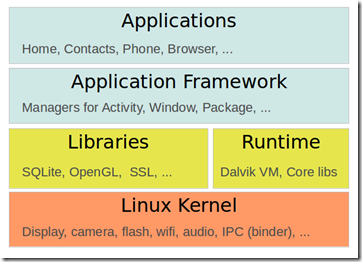
\includegraphics[width=0.7\linewidth]{Images/arch}
    \end{figure}
\end{frame}

\begin{frame}{Requerimientos técnicos}
\begin{itemize}
    \item Java Developer Kit (8)
    \item Android Studio (Android SDK)
    \item Windows, Linux. Mac OS
    \item Simulador (Oficial/Genymotion) ó Telefono
\end{itemize}
\end{frame}

\begin{frame}{Términos útiles}
\begin{itemize}
    \item Android Software Development Kit (Android SDK)
    \item Android debug bridge (adb)
    
    \item Android Virtual Device (AVD) 
    \item Android RunTime (ART)
    \item Dalvik VM
\end{itemize}
\end{frame}

\begin{frame}{Requerimientos desarrollador}
    \begin{itemize}
        \item Programación orientada a objetos
        \item Conocimientos básicos Java
        \item Conocimientos diseño de UI/UX
         \item Ingles
    \end{itemize}
\end{frame}


\begin{frame}{¿Java?}
         \begin{columns}[T] % contents are top vertically aligned
        \begin{column}[T]{5cm} % each column can also be its own environment
    \begin{itemize}
    \item Apache Harmony    
    \item Java - java.util.*, java.io.*, java.lang.* . . .
    \item UI - android.widget.*, android.view.*, android.graphics.*
    \item Tel/SMS - android.telephony.*
    \item OpenJDK
\end{itemize}
        \end{column}
        \begin{column}[T]{5cm} % alternative top-align that's better for graphics
            \begin{figure}
                \centering
                
\includegraphics[width=\linewidth]{Images/dalvik}
            \end{figure}
            
        \end{column}
    \end{columns}
    

\end{frame}

\begin{frame}{Java}
    \begin{figure}
        \centering
        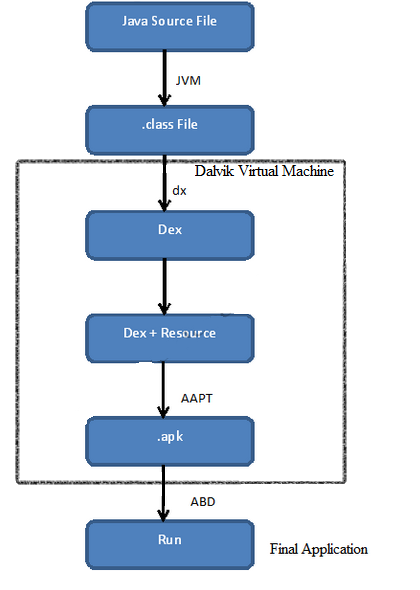
\includegraphics[width=0.55\linewidth]{Images/javatodalvik}
    \end{figure}
\end{frame}


\section{Aplicaciones}
\begin{frame}{Aplicación Android}
    \begin{itemize}
        \item AndroidManifest.xml
        \item Activities
        \item Views
        \item Layouts
        \item Intent \& Intent Redirect
        \item Services
        \item Notifications
        \item Content providers
        \item R file
    \end{itemize}
\end{frame}

\begin{frame}{Aplicaciones Android}
    \begin{itemize}
        \item AndroidManifest.xml
         \item build.graddle
        \item Activities
        \item Views \& Layouts
                \begin{itemize}
            \item Drawable
            \item Layout
            \item Menu
            \item \textbf{Values}
        \end{itemize}
        \item Intent \& Intent Redirect
        \item Services
        \item Notifications
        \item Content providers
        \item R file
    \end{itemize}
\end{frame}


\begin{frame}{Manifest file}
    Configuración de tu aplicación Android
    \begin{itemize}
        \item Datos generales
        \item Iconos
        \item Iconos
    \end{itemize}
\end{frame}

\begin{frame}{build.gradle}
    Tareas de compilación y producción de la aplicación
    
\end{frame}

\begin{frame}{Activities}
    \large
    Activity: Usualmente una pantalla en una aplicación
\end{frame}


\begin{frame}
    \huge
    Demo
\end{frame}


\begin{frame}{Tambien ver}
    \begin{itemize}
        \item \href{https://www.edx.org/course/java-fundamentals-android-development-galileox-caad001x}{Java Fundamentals for Android edx.org}
        \item \href{https://www.edx.org/course/java-fundamentals-android-development-galileox-caad001x}{Desarrollo de aplicaciones profesionales Android edx.org}
    \end{itemize}
\end{frame}

\section{Fin}
\begin{frame}{Gracias}
\begin{itemize}
\item me@vorozco.com
\item http://vorozco.com
\item http://github.com/tuxtor/slides
\end{itemize}
\begin{center}

\includegraphics[width=0.1\linewidth]{Images/cclogo}
\\
This work is licensed under a Creative Commons Attribution-ShareAlike 3.0 Guatemala License.
\end{center}
\end{frame}
\end{document}

